\section{提案手法} \label{sec:ProposedMethod}

提案手法は、文書・文間及びカテゴリ間の関係を考慮した
レーティング予測の手法である。
提案手法では、パラグラフベクトルによってレビューの文書及び各文の
意味表現を生成し、それらをニューラルネットワークによる分類器入力として
レーティング予測を行う。
以下にその基礎となる考えと具体的なアルゴリズムを示す。


\subsection{文書・文間及びカテゴリ間の関係の考慮}

先行研究\cite{fujitani15}の実験結果から、
レビュー内の文毎の素性を元にレビューの分類を行うことが
正答率の向上に有効であると考えられる。
また、カテゴリ間の繋がりの変化が正答率に影響していることから、
これをパラメータとして機械学習のモデルに組み込めば
正答率を向上させることができると考えられる。
さらに、レビュー内の文毎に意味表現を生成し分類器の入力とすれば、
その位置関係を考慮した学習を行うことができる。

以下に、文の位置関係が重要となる例を示す。
2つ目の例は、1つ目の例の2つ目の文と3つ目の文を入れ替えたものである。
\begin{addmargin}{8ex}
  \vspace{1em}
  \setstretch{1}
  食事が美味しかった。 \\
  \textbf{とても良かった。} \\
  部屋から眺めが素晴らしかった。
\end{addmargin}
\begin{addmargin}{8ex}
  \vspace{1em}
  \setstretch{1}
  食事が美味しかった。 \\
  部屋から眺めが素晴らしかった。 \\
  \textbf{とても良かった。}
\end{addmargin}
1つ目の例では、「とても良かった。」という文が直前の食事に関する文の
意味を補完しているのに対し、
2つ目の例では、部屋に関する文の意味を補完している。
このように、文の位置関係によってどの文がどの文と強く関連しているかが変化する。
それによって、予測すべきレビュー全体のレーティングも変化すると考えられる。
このように、文の位置関係の考慮はレーティング予測において重要であると
考えられる。

次に、カテゴリ間の関係が重要となる例を
図\ref{fig:RelationsAmongRatingCategories}に示す。
図\ref{fig:RelationsAmongRatingCategories}のように
「総合」カテゴリのレーティングは一般に他のカテゴリのレーティングに応じて
高くなる。
このような関係は「立地」と「部屋」、「食事」と「サービス」等の
他のカテゴリ間にも存在する。
よって、このことからも、カテゴリ間の関係をレーティング予測において
考慮することで、正答率を向上させられると考えられる。

\begin{figure}
  
\includegraphics[0.3]{fig/relations_among_rating_categories.pdf}
  \caption{カテゴリ間の関係の例}
  \label{fig:RelationsAmongRatingCategories}
\end{figure}

しかし、個々のレビューに対して全ての文ベクトルを
ニューラルネットワークによる分類器の入力とすることは問題がある。
なぜならば、文の数はレビュー毎に異なっており、
複数レビュー内の複数の文ベクトルを単純な行列として表せないためである。
これは、分類器のミニバッチ方式の訓練を難しくし、
プログラムの実行時間を増加させる。
この問題に対処するため、本手法では各レビュー内の文ベクトルに対して
重み付け平均を行う。
これにより、全てのレビューで文ベクトルの数が統一され、
複数レビュー内の複数の文ベクトルをまとめて3次元行列として表すことができる。
つまり、ミニバッチ方式の訓練における計算が容易となる。

分類器はニューラルネットワークを用いて構成することによって、
文書・文間の関係とカテゴリ間の関係を同時に考慮した分類を行う。
従来手法\cite{nal14,rie14,duyu15}では、
分類器として畳込み\nn と全結合\nn が用いられている。
しかし、提案手法においては畳み込みニューラルネットワークより
全結合\nn を用いた方が正答率が高かったため、分類器には後者のみを用いた。


\subsection{アルゴリズム}

\begin{figure}
  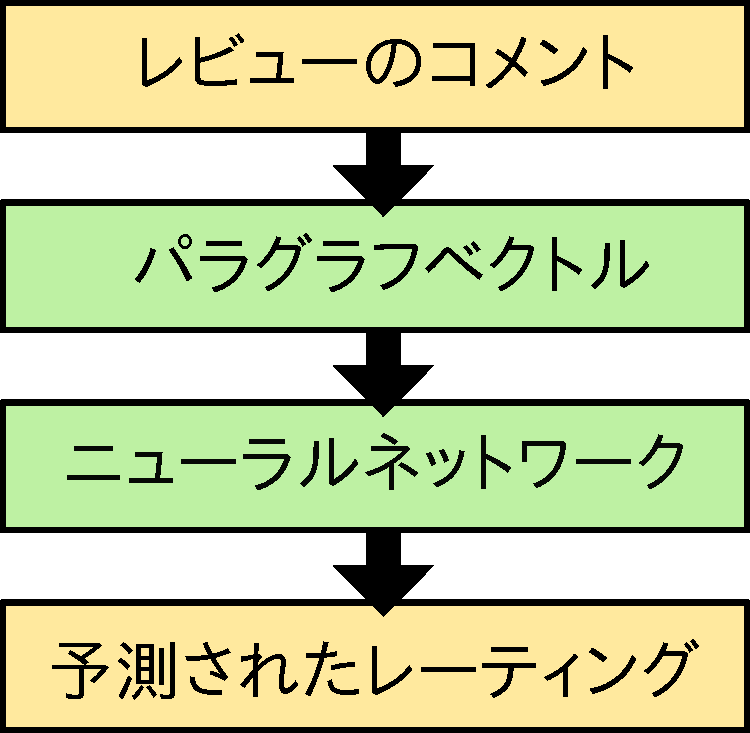
\includegraphics[0.5]{fig/algorithm.pdf}
  \caption{提案手法におけるアルゴリズムの概略}
  \label{fig:MyAlgorithm}
\end{figure}

提案手法のレーティング予測の流れを説明する。
図\ref{fig:MyAlgorithm}にアルゴリズム全体の概略を示す。
提案手法では、PV-DMによってレビュー内の文書全体及び各文の意味表現を
生成し、それらをニューラルネットワークによる分類器の入力として
レーティング予測を行う。
%文毎の意味表現を用いることで文同士の位置関係を考慮し、
%ニューラルネットワークによる分類器を用いることで
%文間及びカテゴリ間の深い関係性を捉えることを目指す。
%提案手法の入力はレビューである文書と正解レーティングの組の集合、
%出力は各文書について予測されたカテゴリ毎のクラスである。
%以下に提案手法の処理の流れを示す。

初めに、PV-DMを用いて、
各レビューの文書全体のベクトルとそれに含まれる各文のベクトルを生成する。
以降、これらをそれぞれ文書ベクトル、文ベクトルと呼ぶ。
文書ベクトルと文ベクトルについては別々に学習し生成する。
%式\ref{eq:PVObjective}に示す目的関数$L_d$を最大化するように学習を行う。
%\begin{multline}
%  L_d = \sum^{T}_{t = n + 1} \{ \log \sigma(s(w_t, w_{t-n}, ..., w_{t-1}, d)) \\
%        + \sum^{k}_{w_{t}' \sim P_n}
%        \log(1 - \sigma(s(w_{t}', w_{t-n}, ..., w_{t-1}, d))) \},
%    \label{eq:PVObjective} \\
%\end{multline}
%\begin{gather}
%  s(w_t, w_{t - n}, ..., w_{t - 1}, d)
%    = W_{map}(w_t)
%      \cdot \begin{bmatrix} W(w_{t - n}) \\ \vdots
%      \\ W(w_{t - 1}) \\ D(d) \end{bmatrix} \nonumber
%\end{gather}
%ここで、$T$は現在の文章内の単語数、$t$は現在の単語位置、$d$は現在の文章、
%$w_i$は位置$i$にある単語、$n$はウィンドウサイズである。
%$W(w_i)$は単語$w_i$に相当する単語ベクトルを単語行列$W$から抜き出す関数を表す。
%$D(d)$は文章$d$に相当する文章ベクトルを文章行列$D$から抜き出す関数を表す。
%関数$s(w_t, w_0, ..., w_n, d)$はある単語とそれが出現する文脈との類似度を
%計算する。
%行列$W_{map}$は内積によって文脈と単語との類似度を計算するための単語毎
%のベクトルを保持する。
%文章行列内の各文章ベクトルはレビュー全体を表す文書ベクトル、または、
%各レビュー内の文ベクトルを表す。
%$\sigma$はシグモイド関数である。
%また、式\ref{eq:PVObjective}の中括弧内の右項はネガティブサンプリングを
%表す。
%ネガティブサンプリングとは、文脈外の単語をデータセットにおける出現確率で
%サンプリングし、それらと文脈の意味が遠ざかるように学習する手法である。
%$w_{t}' \sim P_n$は文脈外の単語$w_{t}'$を単語の出現頻度$P_n$によって
%サンプリングすることを示す。
%ただし、出現頻度は極端に頻出する単語の影響を抑えるため
%各単語に対して3/4乗している。
%現在の単語と同じ単語や同一回の学習で一度サンプリングされた単語は
%サンプリングしない。
式\ref{eq:ParagraphVector}の目的関数における$h$には
引数のベクトルを結合する関数を用いる。
また、学習の高速化のため、Quocら\cite{quoc14}によって
用いられている階層的softmax関数の代替としてネガティブサンプリングを行う。
ネガティブサンプリングとは、文脈外の単語をデータセットにおける出現確率で
サンプリングし、それらと文脈の意味が遠ざかるように学習する手法である。
ただし、出現頻度は極端に頻出する単語の影響を抑えるため
各単語に対して3/4乗している。
現在の単語と同じ単語や同一回の学習で一度サンプリングされた単語は
サンプリングしない。

次に、各レビュー内の全ての文ベクトルに対して重み付け平均を行い、
圧縮された文ベクトルを生成する。
この過程により、各レビューで疎らだった文の数を統一する。
式\ref{eq:WeightedAverageSV}に重み付け平均によって圧縮した
文ベクトル$t_{i_{part}}$を示す。
各文ベクトルは圧縮後の各文ベクトルと位置が近いほど重みが大きくなるように
重み付け平均する。
\begin{gather}
  \mathbf{t}_{i_{part}} = \sum_{i_{sent}}
                          \frac{w(x_{i_{part}}(i_{sent}))}
                               {|\sum_{i_{sent}'}
                                w(x_{i_{part}}(i_{sent}'))|}
                          \mathbf{s}_{i_{sent}},
  \label{eq:WeightedAverageSV} \\
  x_{i_{part}}(i_{sent}) = \frac{i_{sent}}{\#sent - 1}
                           - \frac{i_{part}}{\#part - 1}, \nonumber \\
  w(x) = \begin{cases}
    \frac{1}{2} (\cos(\pi|x|) + 1) & \text{if $|x| \leq 1$} \\
    0 & \text{otherwise}
  \end{cases} \nonumber
\end{gather}
ここで、$\mathbf{s}_{i_{sent}}$はレビュー内の文ベクトル、
$\mathbf{t}_{i_{part}}$は重み付け平均された文ベクトルである。
$i_{sent}$はレビュー内の文ベクトルのインデックス、
$i_{part}$は重み付け平均された文ベクトルのインデックスである。
$\#sent$はレビュー内の文ベクトルの数、
$\#part$は重み付け平均された文ベクトルの数である。
\footnote{
  重み付けの関数には$\cos$関数の他に、
  $x$に対して線形に重みを減少させるような関数や、
  単純に文を区画毎に平均するような関数も考えられる。
  区画毎に平均する関数は他の2つより正答率が低く、線形な関数と
  $\cos$関数はほぼ同じ正答率を示したため、$\cos$関数を採用した。
}

最後に、分類器によってレーティング予測を行う。
分類器は全結合ニューラルネットワークによって構成される。
図\ref{fig:MyModel}に各層の結合の様子を示す。
\begin{figure}
  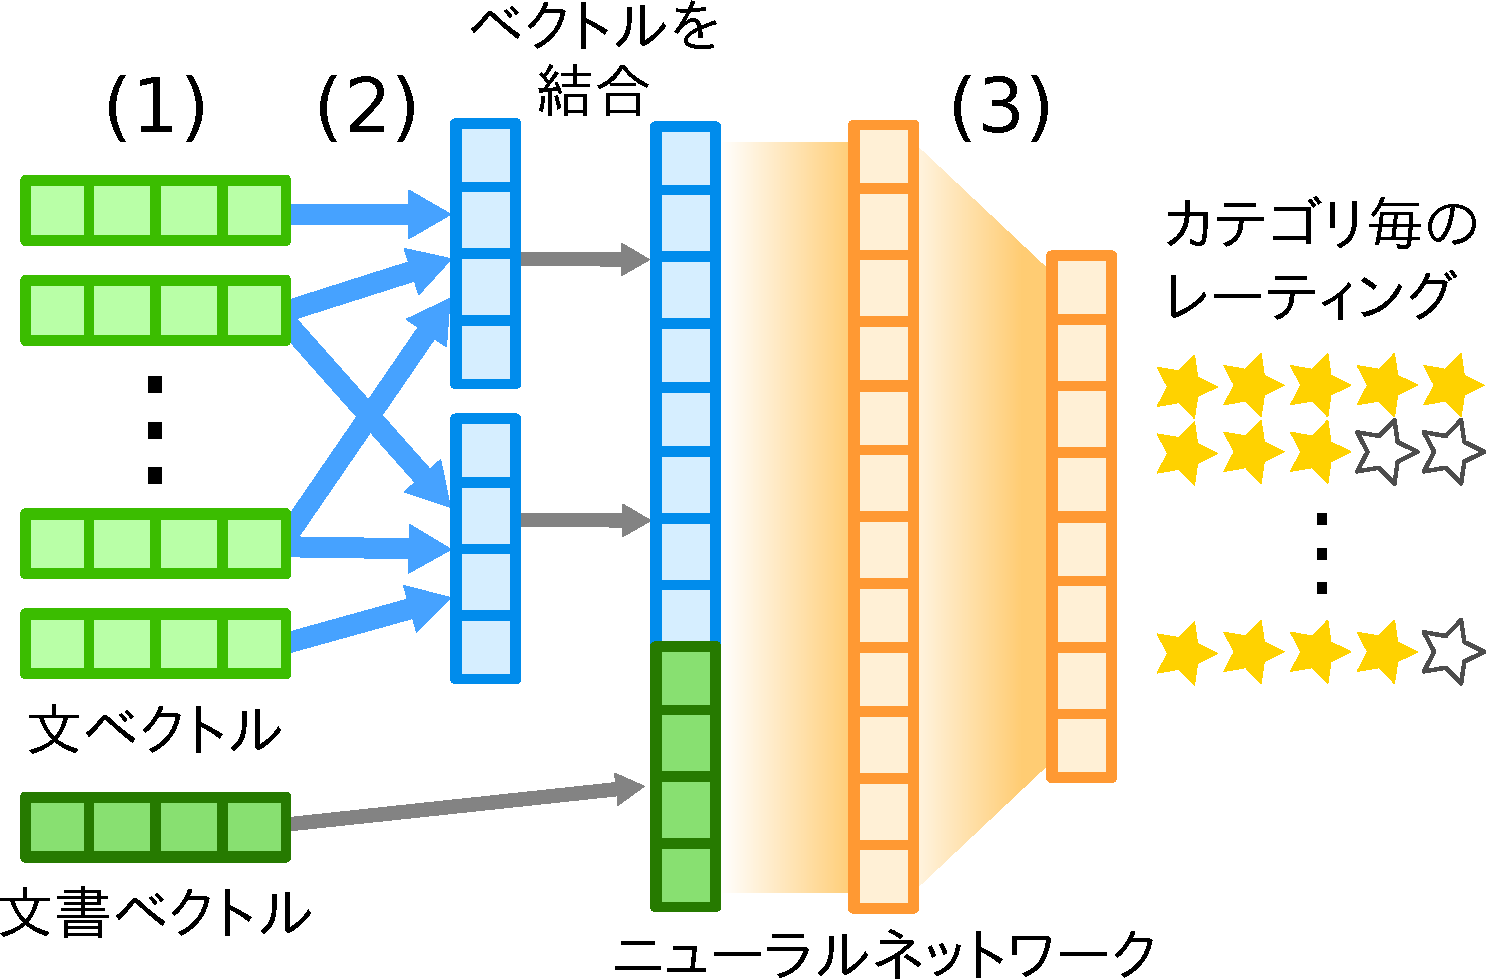
\includegraphics[0.6]{fig/model_with_formal_process_numbers.pdf}
  \caption{全結合ニューラルネットワークによる分類器}
  \label{fig:MyModel}
\end{figure}
入力層はレビュー毎の文書ベクトルと圧縮された文ベクトルの結合ベクトルである。
ニューラルネットワークの活性化関数には、シグモイド関数を用いる。
また、出力層はカテゴリの数とレーティングの場合の数の積だけのニューロンを持ち、
各ニューロンの出力はあるカテゴリがあるレーティングであることの
正規化されていない対数確率を表す。
各ニューロンの出力はカテゴリ毎に交差エントロピー誤差関数によって
損失に変換される。
ニューラルネットワークは式\ref{eq:NNObjective}に示す目的関数$E$を
最小化するように学習を行う。
\begin{gather}
  E = - \sum^{N}_{n = 1} \sum^{C}_{c = 1} \sum^{K}_{k = 1}
        d_{nck} \log{y_{ck}(x_n; w)},
  \label{eq:NNObjective} \\
  y_{ck}(x_n; w) = \frac{e^{u_{ck}(x_n; w)}}
                        {\sum^{K}_{j = 0} e^{u_{cj}(x_n; w)}} \nonumber
\end{gather}
ここで、$u_{ck}$は出力層のニューロンの出力値、$y_{ck}$はカテゴリ$c$において
クラス$k$が選ばれる確率、$w$はニューラルネットワークのパラメータである。
$d_{nck}$は$n$番目の文書がカテゴリ$c$でクラス$k$ならば1、
それ以外で0となる値である。
$N$はミニバッチサイズ、$C$はカテゴリの総数、$K$はクラスの総数である。
ニューラルネットワークによる多値分類では一般に、
出力層のニューロンの出力値全体をsoftmax関数で
正規化する。
しかし、複数カテゴリの多値分類問題において、
同様に出力層のニューロンの出力値を正規化してしまうと
softmax関数の値が確率としての意味を成さない。
よって、式\ref{eq:NNObjective}では、
カテゴリ毎にsoftmax関数でニューロンの出力値が示す対数確率を正規化する。
そして、それらを各カテゴリ毎の目的関数とし足し合わせることで
あるレビューに対する目的関数を構成する。
これを全てのレビューに対して足し合わせ、
ニューラルネットワークの目的関数とする。
さらに、ニューラルネットワークの学習時にはドロップアウト及び重み減衰を行う。
ただし、重み減衰において全結合層の重みの内、バイアスは減衰していない。
パラメータ最適化の手法にはAdam\cite{diederik15}を用いる。
